	\section{Цель работы}
		Решение 2х-мерной задачи симуляции жидкости (газа) методом решеточных уравнений Больцмана.
		
		Матрица задачи должна занимать в памяти не менее 100 Мб на каждое процессорное ядро, задействованное в вычислениях, верхний предел – 1Гб на ядро. По возможности использовать при решении специализированные функции MPI: $ MPI\_Sendrecv\_replace $, $  MPI\_Reduce $.
		
	\clearpage
	\section{Порядок выполенения работы}
	
		\subsection{Описание алгоритма}
			Методы решёточных уравнений Больцмана — класс методов вычислительной гидродинамики для моделирования жидкостей. Методы решёточных уравнений Больцмана удобны благодаря их концептуальной и вычислительной простоте, их использование ограничено малыми скоростями и тем, что метод обладает неустойчивым поведением на границе подвижных тел.
			
			Основная идея состоит в том, что газы / жидкости можно представить как состоящие из большого числа мелких частиц. Обмен импульсом и энергией достигается за счет распространения частиц и столкновения (коллизии) с другими частицами по принципу бильярда. Этот процесс может быть смоделирован по уравнению переноса Больцмана:
			
			\[ \dfrac{\partial f}{\partial t} +\vec{u}\triangledown f = \Omega ,\]
			
			где $ f(\vec{x},t) $ - функция распределения частиц, $ \vec{u} $ - скорость частицы, a $ \Omega $ - оператор коллизии. LBM упрощает оригинальную идею Больцмана о газовой динамике, уменьшая количество частиц и ограничивая их узлами решетки. Для двумерной модели частица ограничена потоком в возможном из 9 направлений, в том числе оставаясь в покое. Эти скорости называются микроскопическими скоростями и обозначаются через $ \vec{e_i} $, где $ i = 0,... , 8 $. Эта модель широко известна как модель D2Q9, поскольку она двумерна и включает в себя 9 векторов скорости. На рисунке 1 показан типичный узел решетки D2Q9-модели с 9 скоростями $ \vec{e_i} $, определяемый формулой
			
			\begin{equation*}
				\vec{e_i} = 
				\begin{cases}
					(0,0) &i = 0\\
					(1, 0),(0, 1),(-1, 0),(0, -1) & i = 1, 2, 3, 4\\
					(1, 1),(-1, 1),(-1, -1),(1, -1) & i = 5, 6, 7, 8
				\end{cases}
			\end{equation*}
			
			С каждой частицей на решетке мы связываем дискретную функцию распределения вероятностей $ f_i (\vec{x},\vec{e_i}, t) $ или просто $ fi (\vec{x}, t), i = 0. , , 8, $, которая описывает вероятность распространения в одном конкретном направлении.
		
			\begin{figure}[h]
				\centering
				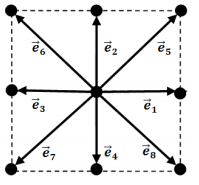
\includegraphics[width=0.2\linewidth]{d2q9}
				\caption{Иллюстрация узла решетки модели D2Q9}
				\label{fig:d2q9}
			\end{figure}
		
			Макроскопическая плотность жидкости определяется как суммирование микроскопической функции распределения частиц,
					\[ \rho(\vec{x},t) = \sum_{i=0}^8 f_i(\vec{x}, t) .\]
					
			Соответственно, макроскопическая скорость $\vec{u}(\vec{x},t) $ представляет собой среднее значение микроскопических скоростей $ \vec{e_i} $, взвешенных функциями распределения $ f_i $,
			
			\[ \vec{u}(\vec{x},t) = \frac{1}{\rho} \sum_{i=0}^8 c~f_i~\vec{e_i}.\]
			
			Ключевыми шагами в LBM являются процессы распространения и столкновения , описанные следующим выражением:
			
			\[f_i(\vec{x}+c~\vec{e_i}~\vartriangle t, t+\vartriangle t) - f_i(\vec{x}, t) = \dfrac{[f_i(\vec{x}, t) - f_i^{eq}(\vec{x}, t)]}{\tau},\]
			
			где $ f_i^{eq}(\vec{x}, t) $ - равновесное распределение, а $ \tau $ рассматривается как время релаксации к локальному равновесию.
			
			При фактической реализации модели потоки и столкновение вычисляются отдельно, и особое внимание им уделяется при работе с узлами на границе решетки. На рисунке  графически показано, как выполняется этап распространения для внутренних узлов.
	
			\begin{figure}[h]
				\centering
				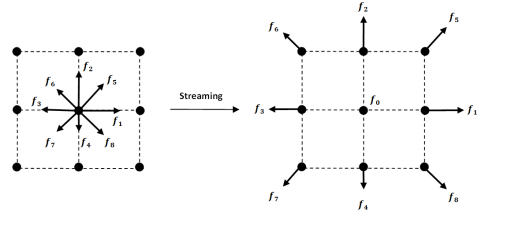
\includegraphics[width=0.6\linewidth]{images/streaming}
				\caption{Иллюстрация процесса распространения частиц узла решетки}
				\label{fig:streaming}
			\end{figure}
			
			Равновестное распределение вычисляется по формуле 
			
			\[ f_i^{eq}(\vec{x}, t) = w_i\rho+\rho s_i(\vec{u}(\vec{x},t)) ,\]
			
			где $ s_i(\vec{u}) $ вычисляется как
			\[ s_i(\vec{u}) =w_i[3 \dfrac{\vec{e_i} \vec{u}}{c} + \frac{9}{2}\dfrac{(\vec{e_i} \vec{u})^2}{c^2} - \frac{3}{2} \dfrac{\vec{u} \vec{u}}{c^2}],\]
			
			а $ w_i $, вес, определён как
						\begin{equation*}
			w_i = 
			\begin{cases}
			4/9 &i = 0\\
			1/9 & i = 1, 2, 3, 4\\
			1/36 & i = 5, 6, 7, 8
			\end{cases}
			\end{equation*}
			
			а $ c = \dfrac{\vartriangle x}{\vartriangle t} $ - скорость решетки.
			
			Общий алгоритм выглядит следующим образом:
			\begin{enumerate}
				\item Инициализация $ f_i $
				\item Шаг распространения $ f_i \rightarrow f_i^*$ в направлении $ \vec{e_i} $ \label{it:str}
				\item Вычисление макроскопических $ \rho $ и $ u $ из $ f_i^* $.
				\item Вычисление $ f_i^{eq} $
				\item Шаг столкновения частиц: $ f_i=f_i^*-\dfrac{1}{\tau}(f_i^* - f_i^{eq}) $ \label{it:col}
				\item Повторить \ref{it:str} - \ref{it:col}
			\end{enumerate}
			
		\subsection{Начальные условия}
		В качестве начальных условий выбрана воронка из частиц, распределённых равномерно, с радиусом в центре пространства.		Пространство ограничено стеной, от которой частицы отскакивают.	
		
		\begin{figure}[ht]
			\begin{minipage}[ht]{0.49\linewidth}
				\center{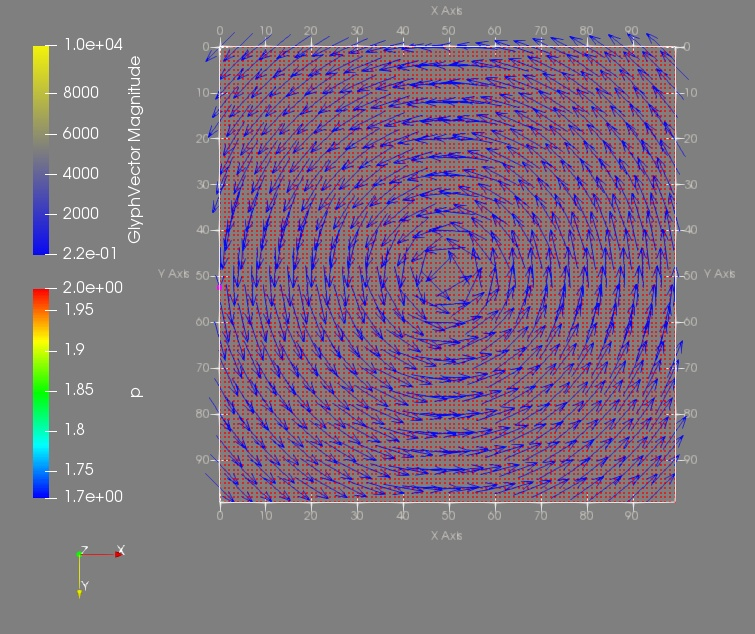
\includegraphics[width=0.8\linewidth]{0000}\textbf{\\ ~}}
			\end{minipage}
			\hfill
			\begin{minipage}[ht]{0.49\linewidth}
				\center{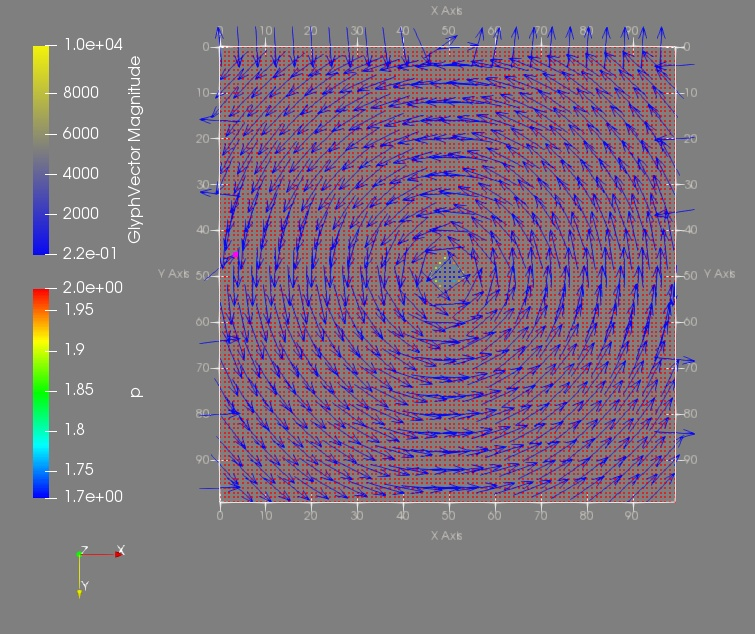
\includegraphics[width=0.8\linewidth]{0001}\\ ~}
			\end{minipage}
			\vfill
			\begin{minipage}[ht]{0.49\linewidth}
				\center{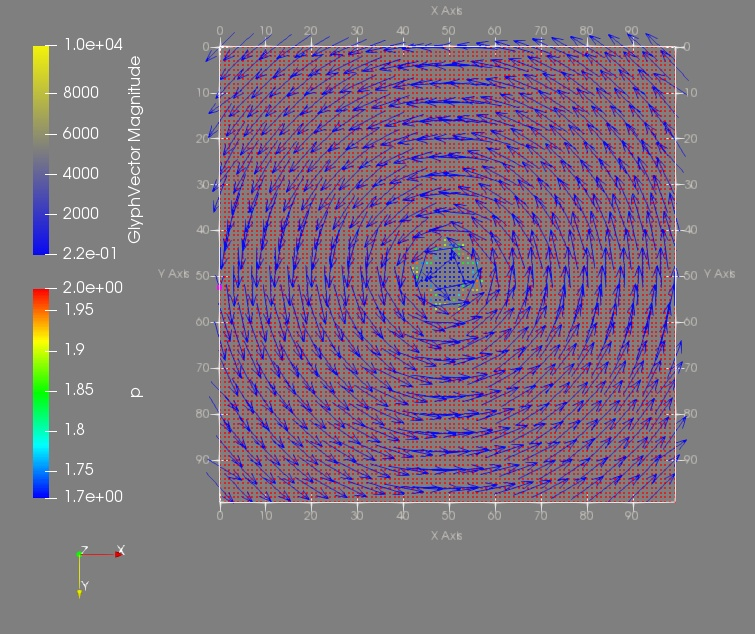
\includegraphics[width=0.8\linewidth]{0002}\\ ~}
			\end{minipage}
			\hfill
			\begin{minipage}[ht]{0.49\linewidth}
				\center{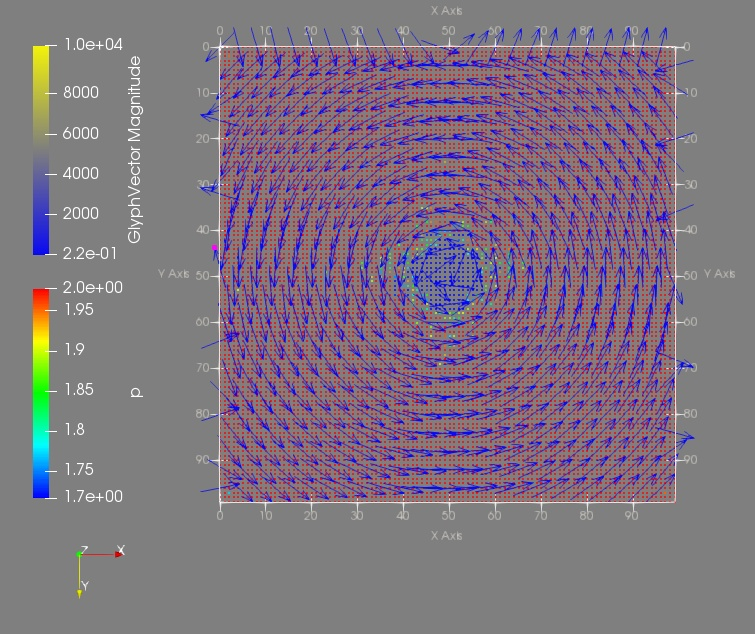
\includegraphics[width=0.8\linewidth]{0003} \\ ~ }
			\end{minipage}
			\vfill
			\begin{minipage}[ht]{0.49\linewidth}
				\center{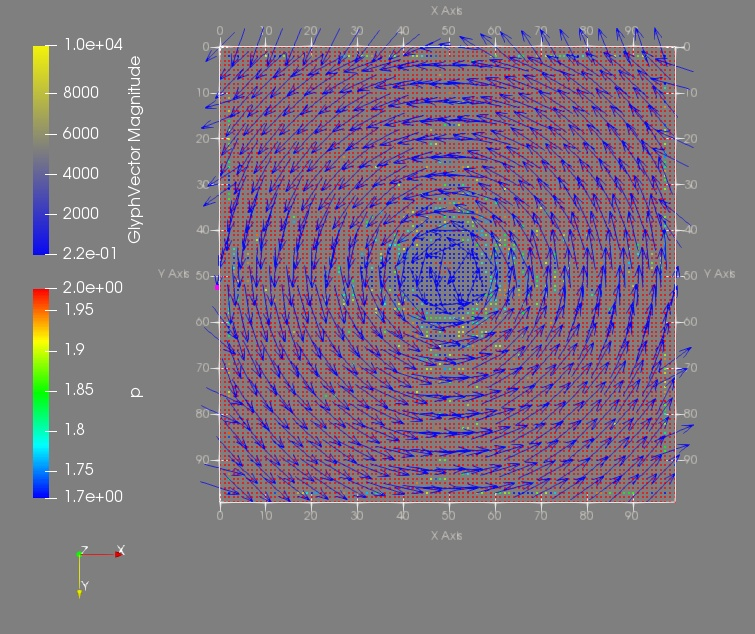
\includegraphics[width=0.8\linewidth]{0004}\\ ~}
			\end{minipage}
			\hfill
			\begin{minipage}[ht]{0.49\linewidth}
				\center{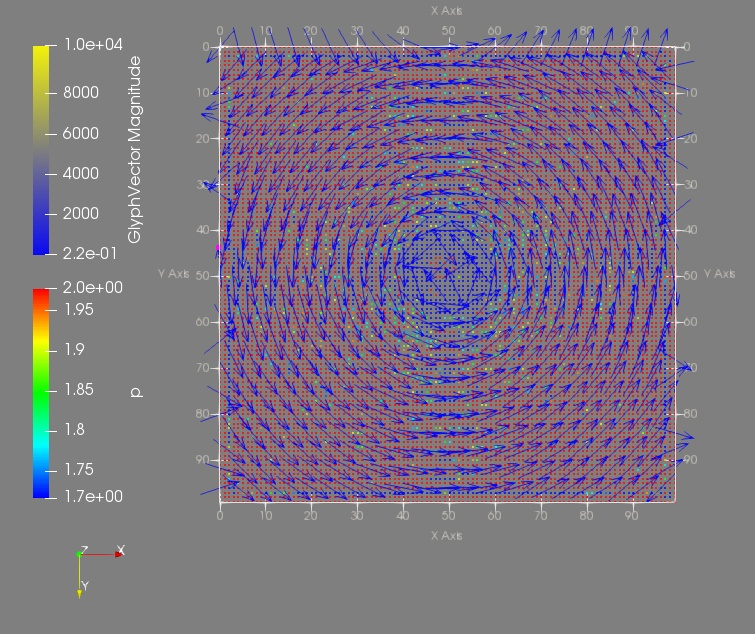
\includegraphics[width=0.8\linewidth]{0005}\\ ~}
			\end{minipage}
			\vfill
			\begin{minipage}[ht]{0.49\linewidth}
				\center{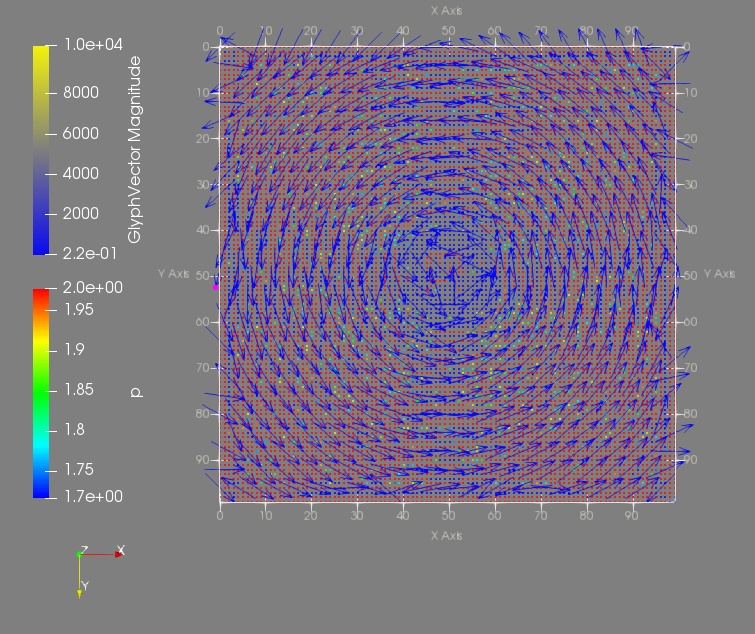
\includegraphics[width=0.8\linewidth]{0006}\\ ~}
			\end{minipage}
			\hfill
			\begin{minipage}[ht]{0.49\linewidth}
				\center{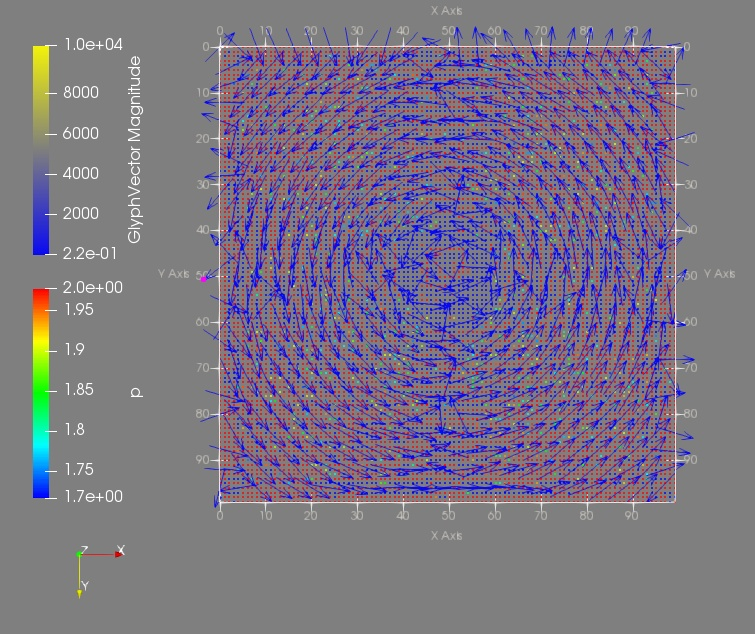
\includegraphics[width=0.8\linewidth]{0007}\\ ~}
			\end{minipage}
			\vfill
			\caption{Пример симуляции для $ c=1, \tau = 0.8 $.}
			\label{fig:example}  
		\end{figure}
			
		\FloatBarrier
		\subsection{Методика распараллеливания}
			Процессор с 0 индексом резервируется для сохранения состояний сетки в каждый момент времени.
			
			Каждый процессор до этапа распространения обменивается с процессорами со смежными частями сетки своими нижней и верхней строкой методом $ MPI\_Sendrecv\_replace $. Далее каждый процессор производит шаги распространения и столкновения. 
			
			Раз в заданное количество шагов нулевой узел собирает данные функцией $ MPI_Gatherv $ из вычисляющих процессоров и сохраняет их в $ *.csv $ файл. 
			
		\subsection{Исследование производительности реализованного алгоритма}
			
			Метод решеточных уравнений Больцмана требует $ O(n^2 * t) $ арифметических операций, где $ t $ - время симуляции. Тогда производительность метода можно оценить формулой $  \dfrac{n^2 * t}{\tau} $, где $ \tau $ - время выполнения алгоритма. На основе таблицы результатов \ref{t1} составлен график зависимости производительности от количества процессоров \ref{fig:performance}. Вычисления выполнялись при $ t=100 $.
			
%			Как видно из графика \ref{fig:performance}, увеличение производительности с ростом количества процессоров близко к линейному.
			\clearpage	
		
			\begin{table}
				\centering
				\caption{Результаты вычислений, где $ P $ - количество процессоров, $ n $ - размер сетки, $ \tau $ - время выполнения.}
				\label{t1}
				\csvreader[tabular=|l|r|l|c|,
				table head=\hline & P & n & $ \tau $\\\hline,
				late after line=\\\hline]%
				{listings/data.csv}{numberOfProcessors=\pnumber,equationCount=\n,allRounds=\ftime}%
				{\thecsvrow & \pnumber& \n & \ftime }%
			\end{table}
		
			\begin{figure}
				\centering
				\begin{tikzpicture}
					\begin{axis}[ylabel=Производительность, xlabel=Количество процессоров, xtick={0,2,4,6,8,12,16,20,24}]
						\addplot table [x=numberOfProcessors, y expr=(\thisrow{equationCount}^2*100)/(\thisrow{allRounds}), col sep=comma] {listings/data.csv};
					\end{axis}
				\end{tikzpicture}
				\caption{Зависимость производительности алгоритма от количества процессоров.} \label{fig:performance}
			\end{figure}
	
	\FloatBarrier
	\clearpage	
	\section{Вывод}
		В ходе работы
		\begin{enumerate}
			\item Реализован метод решеточных уравнений Больцмана с задаными ограничениями на начальные данные.
			\item Проанализирована производительность алгоритма.
			\item Получены навыки работы с программой для визуализации данных ParaView.
		\end{enumerate}
	
		Исходный код программ доступен по ссылке \href{https://github.com/goto1134/MPI-labs}{https://github.com/goto1134/MPI-labs}.